\documentclass[letterpaper, 12pt]{article}
\usepackage[letterpaper, top=2.5cm, bottom=2.5cm, left=3cm, right=3cm]{geometry} %margenes
\usepackage[utf8]{inputenc} %manejo de caracteres especiales
\usepackage[spanish]{babel} %manejo de encabezados de inglés a español
\usepackage{fancyhdr} %formato de los encabezados de página
\usepackage{ragged2e} %alineado real justficado
\usepackage{graphicx} %manejo de imagenes
\usepackage{amsmath} %manejo de notación matemática
\usepackage{mathtools} %manejo de notación matemática
\usepackage{blindtext} %texto de relleno
\usepackage{cancel} %permite la simbolización de cancelación de terminos
\usepackage{enumitem}[shortlabels] %listas con letras
\usepackage{amssymb} %manejo de simbolog►1a matematica
\usepackage[titles]{tocloft} %manejo de elementos para el índice
\usepackage{float} %manejo de centrado para figuras
\usepackage{hyperref} %manejo d hipervínculos
\hypersetup{%formato de colors de hipervínculos, permite crear pdfs con enlaces a los temas
    colorlinks=true,      
    urlcolor=blue,
    linkcolor=blue
}
\pagestyle{fancy}
\fancyhf{}
\rfoot{\thepage}

\DeclarePairedDelimiter\ceil{\lceil}{\rceil}
\DeclarePairedDelimiter\floor{\lfloor}{\rfloor}

\begin{document}
    
    %PORTADA
    \begin{titlepage}
        \begin{figure}[ht]
            \centering
            
\includegraphics[width=15cm]{logosITT.png}
        \end{figure}
        \centering
        {\scshape\LARGE Tecnológico Nacional de México\\Instituto Tecnológico de Tijuana\par}
        \vspace{1cm}
        {\scshape\Large Cálculo Diferencial\par}
        \vspace{1cm}
        {\scshape\Large Unidad 2\par}
        \vspace{1.5cm}
        {\huge\bfseries Funciones\par}
        \vfill
        Asesor: \par
        C. Abraham Jhared Flores Azcona
        
        \vfill

        {\large \emph{``If it's close enough, it's good enough.''}}


    \end{titlepage}

    \newpage
        \pagestyle{empty}
        \tableofcontents
        \listoffigures

        \newpage
        \pagestyle{fancy}
        \lhead{\textbf{Unidad 2: Funciones}}
        \section{Definición de variable, función, dominio y rango}
        A grandes rasgos, lo que ya tenemos que tener en cuenta para el resto de las matemáticas de alto nivel.
        \begin{itemize}
            \item \textbf{Variable: }valor que cambia. Literalmente, lo que \emph{varía}. Generalmente se acostumbra a usar a \(x\) y a \(y\) como variables.
            \item \textbf{Función: }se dice que \(y\) es \emph{función} de \(x\) cuando a cada valor de la variable \(x\) \emph{corresponden uno o varios valores determinados} de la variable \(y\).
            \item \textbf{Dominio: }son los posibles valores que la \emph{variable independiente} puede tomar.
            \item \textbf{Rango: }son los posibles valores que la \emph{variable dependiente} puede tomar.
        \end{itemize}
        Generalmente, lo que siempre nos piden obtener de una función cualquiera es su dominio y rango, (correspondiente a posibles valores de los ejes \(x\) y \(y\)). De cajón, si nos piden dominio tenemos que asumir que nos están pidiendo los \emph{posibles valores de \(x\)}. Si nos piden rango, nos están pidiendo los \emph{posibles valores de \(y\)}.
        \\\newline
        \textbf{Ejemplo: }
        \\Obtener el \emph{dominio y rango }de la siguiente función
        \[f(x)=x^2-1\]
        \emph{Para el dominio:}
        \\
        En este caso, como \(f(x)\) es un polinómio de 2do. grado (porque \(x\) está elevado al cuadradro), \emph{todos los valores que se le dan a \(x\) producen un valor.} Podemos comprobar haciendo iteraciones (evaluar cierta cantidad de veces), en este caso desde [\(-2,2\)] por intervalos enteros:
        \\\newline
            •Para \(x=-2\):
            \[\begin{matrix}
                f(x)&=&x^2-1\\
                f(-2)&=&(-2)^2-1\\
                f(-2)&=&4-1\\
                f(-2)&=&3
            \end{matrix}\]
            •Para \(x=-1\):
            \[\begin{matrix}
                f(x)&=&x^2-1\\
                f(-1)&=&(-1)^2-1\\
                f(-1)&=&1-1\\
                f(-1)&=&0
            \end{matrix}\]
            •Para \(x=0\):            
            \[\begin{matrix}
                f(x)&=&x^2-1\\
                f(0)&=&0^2-1\\
                f(0)&=&0-1\\
                f(0)&=&-1
            \end{matrix}\]
            •Para \(x=1\):
            \[\begin{matrix}
                f(x)&=&x^2-1\\
                f(1)&=&1^2-1\\
                f(1)&=&1-1\\
                f(1)&=&0
            \end{matrix}\]
            •Para \(x=2\):
            \[\begin{matrix}
                f(x)&=&x^2-1\\
                f(2)&=&2^2-1\\
                f(2)&=&4-1\\
                f(2)&=&3
            \end{matrix}\]
        Con esto se puede deducir que cada intervalo que usemos para \(x\) está definido en \(f(x)\) (nos genera un resultado pues). Entonces:
        \[\text{Para }f(x),\, x\in(-\infty,\infty)\]
        Escrito de otra manera:
        \[\text{Para }f(x),\, x\in \mathbb{R}\]
        \emph{Para el rango:}        \\
        No se acostumbra a pedir debido a que conociendo el dominio, podemos conocer el rango (ya que el rango depende del dominio). Primero recordemos que
        \[f(x)=y\therefore y=x^2-1\]
        Entonces, procedemos a despejar \(x\):
        \[\begin{matrix}
            y&=&x^2-1\\
            y+1&=&x^2\\
            \pm\sqrt{y+1}&=&x\therefore\\
            \therefore\pm\sqrt{y+1}&\geq&0\\
            y+1&\geq&0\\
            y&\geq&-1
        \end{matrix}\]
        Esto nos indica que el rango de \(y\) son todos los valores mayores ó iguales a \(-1\), reescrito en notación de intervalos
        \[\text{Para }f(x),\, f(x)\in[-1,\infty)\]
        \section{Función real de variable real y su representación gráfica}
        Los valores que estaremos manejando (lo cuál se explicó en la unidad 1) son los números reales (\(\mathbb{R}\)). Por lo tanto, las funciones que estaremos manejando aceptan valores de \(\mathbb{R}\).
        Se acostumbra a usar dos rectas de valores infinitos que se intersectan en el punto (\(0,0\)) y que los ángulos que forman son de 90° cada uno. Se conoce como \emph{plano cartesiano}. 
        \begin{figure}[H]
            \centering
            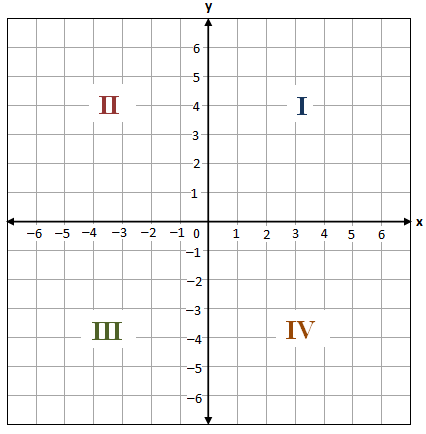
\includegraphics[width=6cm]{plano.png}
            \caption{Plano cartesiano con cuadrantes.}
        \end{figure} 
        De manera similar al documento de la unidad pasada, una buena manera de ilustrar la diferencia de una función con valores en \(\mathbb{R}\) es comparandola con si misma pero con valores en \(\mathbb{N}\). Para referencia, se usará \(f(x)=x^2\) para ámbas gráficas.
        \\\newline
        •Para \(f(x):\mathbb{N}\rightarrow\mathbb{N}\):
        \begin{figure}[H]
            \centering
            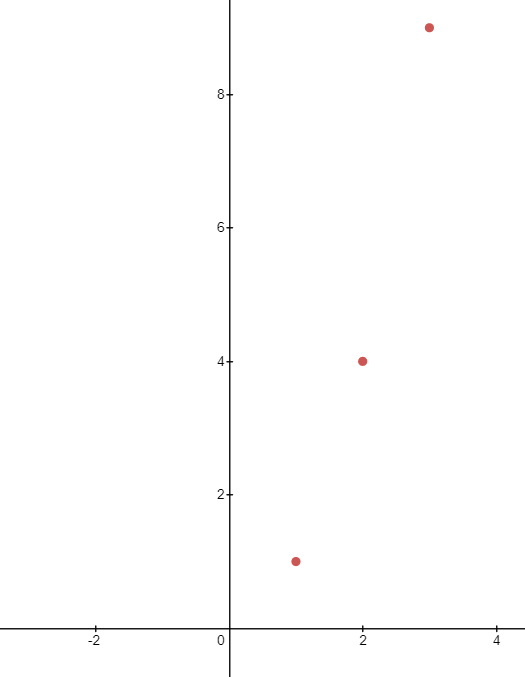
\includegraphics[width=8cm]{fxn.PNG}
            \caption{\(x^2\) usando \(\mathbb{N}\) como dominio y rango.}
        \end{figure}  
        •Para \(f(x):\mathbb{R}\rightarrow\mathbb{R}\):
        \begin{figure}[H]
            \centering
            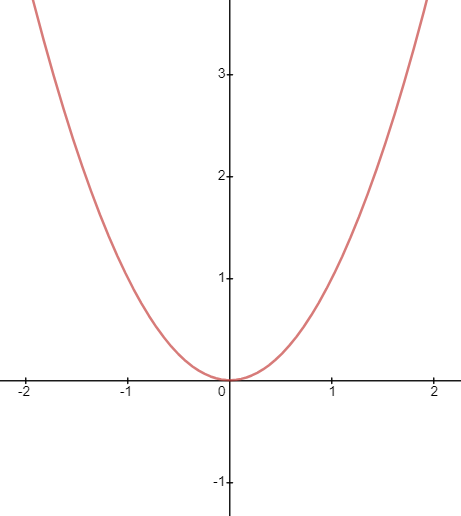
\includegraphics[width=8cm]{fxr.png}
            \caption{\(x^2\) usando \(\mathbb{R}\) como dominio y rango.}
        \end{figure}
        Notese que con \(\mathbb{R}\) tenemos una gráfica más acorde a una parábola, mientras que con \(\mathbb{N}\) nos sale ``mocha''. En otras palabras, \(\mathbb{R}\) nos da un mayor márgen de valores para tener más libertad y mayor presición en nuestros resultados.
        \section{Función inyectiva, suprayectiva y biyectiva}
        Son clasificaciones de funciones, su comportamiento se ilustra de mejor manera con Teoría de Conjuntos.
        \\\newline\textbf{Inyectiva: }los valores de la variable pueden no estar en función de los valores de la variable dependiente. Por decirlo de una manera, \emph{los valores de \(Y\) pueden no estar conectados a los de \(X\) (que cursi)}.
        \begin{figure}[H]
            \centering
            
\includegraphics[width=8cm]{inyective.png}
            \caption{Ejemplo de conjuntos de una función inyectiva.}
        \end{figure} 
        \textbf{Suprayectiva: }los valores de la variable dependiente tienen al menos una conexión con los de la variable independiente. Puede haber mas de una conexión.
        \begin{figure}[H]
            \centering
            
\includegraphics[width=8cm]{surjective.png}
            \caption{Ejemplo de conjuntos de una función suprayectiva.}
        \end{figure}
        \textbf{Biyectiva: }cada valor de la variable dependiente tiene solo una conexión con los de la varaible independiente; ninguno de ellos está solo. Por decirlo de una manera, hay una \emph{``correspondencia uno a uno''}.
        \begin{figure}[H]
            \centering
            
\includegraphics[width=8cm]{biyective.png}
            \caption{Ejemplo de conjuntos de una función biyectiva.}
        \end{figure}
        Cabe destacar que si una función es byectiva, esta tiene una \emph{función inversa}, esto es debido que si \(A\) va a una sola \(B\), y si cada \(B\) tiene una \(A\) correspondiente, entonces podemos decir que el inverso existe.
        \section{Funciones algebraicas: polinomiales y racionales}
        Son dos tipos de funciones, los polinomiales a grandes rasgos son aquellas que revuelven sobre potencias enteras positivas de \(x\). Su forma general es la siguiente:
        \[f(x)=a_nx^n+a_{n-1}x^{n-1}+\dots+a_2x^2+a_1x+a_0\]
        El grado del polinomio es la potencia mayor de \(x\) en la expresión. Entre las polinomiales tenemos:
        \begin{itemize}
            \item \emph{Constante (linea horizontal):} \(f(x)=a=ax^0\).
            \item \emph{Lineal (una linea con inclinicación):} \(f(x)=ax+b\).
            \item \emph{Cuadrática (la parábola):} \(ax^2+bx+c\). 
        \end{itemize}
        Generalmente, estas tienen dominio en \(\mathbb{R}\).
        \\\newline
        Para las funciones racionales, son \emph{las que estan expresadas como razones o cocientes}. Su definición es la siguiente
        \[f(x)=\frac{P(x)}{Q(x)},\,\forall Q(x)\neq 0\]
        Donde \(P(x)\) y \(Q(x)\) son funciones polinomiales que carecen de raices comunes. De manera gráfica, son aquellas que tienen discontinuidades (sus trazos no se conectan). El ejemplo trillado es de \(f(x)=\frac{1}{x}\):
        \begin{figure}
            \centering
            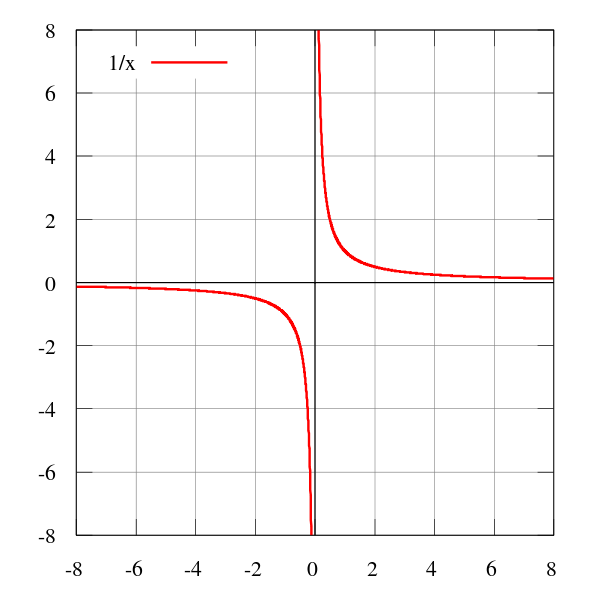
\includegraphics[width=10cm]{1x.png}
            \caption{Gráfica de \(f(x)=\frac{1}{x}\).}
        \end{figure}
        Este tipo de funciones son de sumo interés para nuestro estudio de \emph{límites y continuidad} de la siguiente unidad.
        \section{Funciones escalonadas}
        Un tipo de funciones con un comportamiento especial. Como su nombre implica, la forma gráfica es similar a la de unos escalones; las mas relevantes son dos funciones: \emph{la de suelo y la de piso}:
        \[\begin{matrix}
            \text{Suelo:}&\floor*{x}&=&\text{max}\{n\in\mathbb{Z}|n\leq x\}\\
            \text{Techo:}&\ceil*{x}&=&\text{min}\{n\in\mathbb{Z}|n\leq x\}
        \end{matrix}\]
        A pesar de que se ve complejo, su operación que hacen es bastante simple, \(\floor*{x}\) redondea el valor de \(x\) hacia el valor entero anterior (redondea para abajo) y \(\ceil*{x}\) redondea el valor de \(x\) al valor entero siguiente (redondea para arriba).
        Esto se puede apreciar para sus respectivas gráficas.
        \begin{figure}[H]
            \centering
            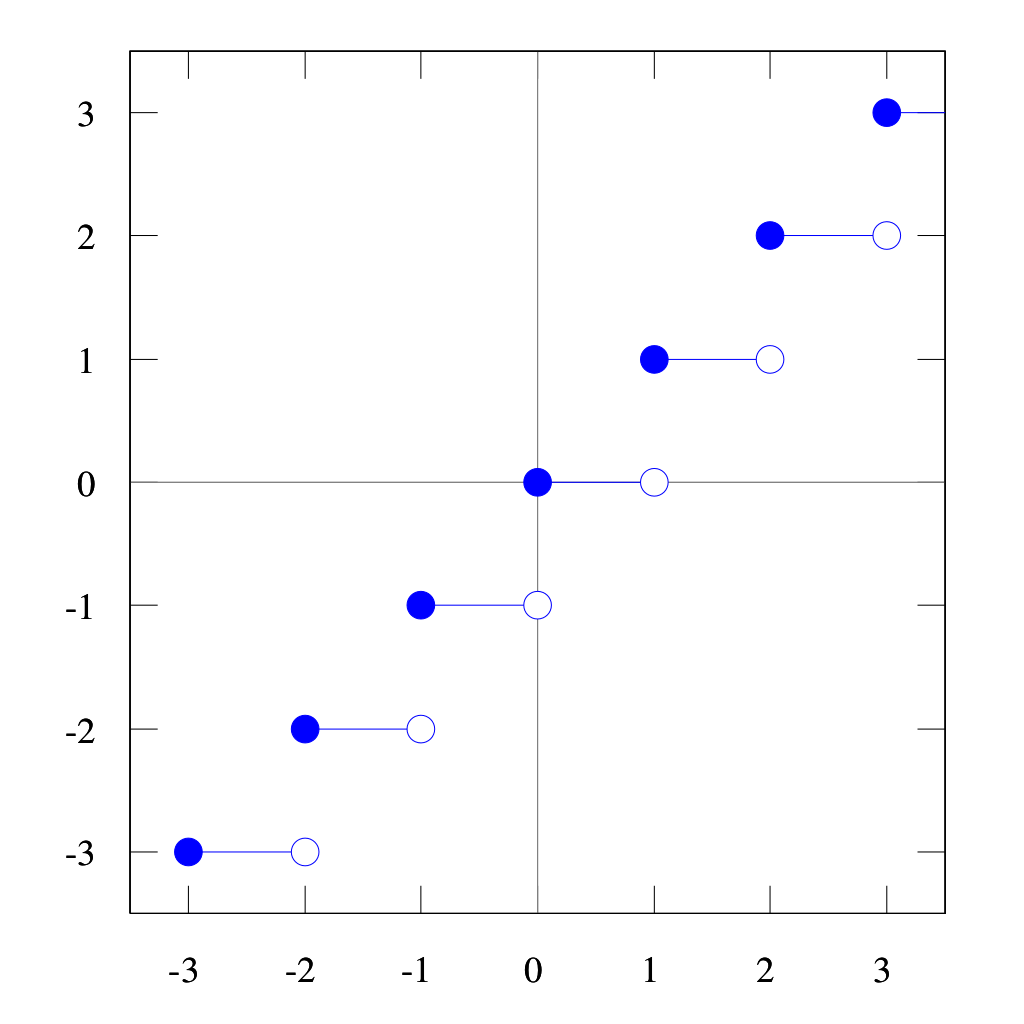
\includegraphics[width=10cm]{suelo.png}
            \caption{Gráfica de la función \(\text{Suelo}\,(x)\).}
        \end{figure}
        \begin{figure}[H]
            \centering
            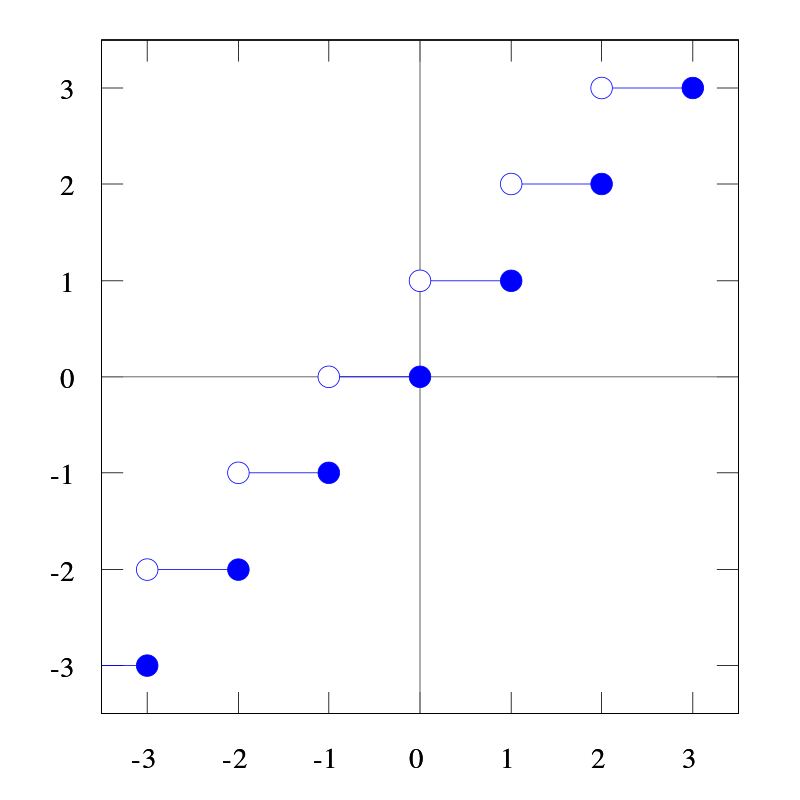
\includegraphics[width=10cm]{piso.png}
            \caption{Gráfica de la función \(\text{Techo}\,(x)\).}
        \end{figure}
        \section{Operaciones con funciones: adición, multiplicación, división y composición}
        Como se indica, son las posibles opreaciones que se pueden hacer entre funciones. Sabiendo las propiedades de las operaciones básicas en numeros reales, podemos hacer dichas opreaciones con funciones con bastante destreza y facilidad. Como referencia, se haran 
        dichas operaciones con \(f(x)=x^2+1\) y \(g(x)=x-1\).
        \\\newline \textbf{Suma: }
        \[f(x)+g(x)=(x^2+1)+(x-1)=x^2+1+x-1=x^2+x\]
        \textbf{Resta: }
        \[f(x)+g(x)=(x^2+1)-(x-1)=x^2+1-x+1=x^2-x+2\]
        \textbf{Multiplicación: }
        \[f(x)\cdot g(x)=(x^2+1)(x-1)=x^2\cdot x-x^2\cdot(-1)+1\cdot x+1(-1)=x^3-x^2+x-1\]
        \textbf{División: }
        \[\frac{f(x)}{g(x)}=\frac{x^2+1}{x-1}\]
        \[\frac{g(x)}{f(x)}=\frac{x-1}{x^2+1}\]
        \textbf{Composición: }es cuando una función va a ser evaluada con otra función. NOTA: \((f\circ g)(x)\neq (g\circ \!f)(x)\) y \((f\circ g)(x)=f(g(x))\).
        \[(f\circ g)(x)=f(g(x))=(x-1)^2+1=(x^2-x-x+1)+1=x^2-2x+1+1=x^2-2x+2\] 
        \[(g\circ \!f)(x)=g(f(x))=(x^2+1)-1=x^2+1-1=x^2\]
        \section{Función implícita}
        A grandes rasgos, cuando nos referimos a una función implícita, nos referimos a que dicha función esta expresada con la variable dependiente e independiente en un lado e igualadas a una constante. Un ejemplo de ello es la ecuación de la circunferencia con \(r=1\):
        \[\begin{matrix}
            \text{Implícita:}&x^2+y^2=1\\
            \text{Explícita (forma común):}&y=\pm\sqrt{1-x^2}
        \end{matrix}\]
        \section{Otro tipo de funciones}
        Como todo, hay otras clasificaciones y un montón de funciones con gráficas interesantes, pero las mas relevantes son las siguientes
        \subsection{Trigonométicas}
        Usadas demasiado para resolver problemas relacionados a la trigonometría e hipotenusas. De cajón, a estas alturas se evaluan en RADIANES. Las mas importantes son:
        \[\begin{matrix}
            \sin x\\
            \cos x\\
            \tan x
        \end{matrix}\]
        De ellas se obtienen las demás acorde a las identidades trigonométicas. Sus inversas son las siguientes:
        \[\begin{matrix}
            \sin ^{-1}x &\text{ó}&\arcsin x\\
            \cos ^{-1}x &\text{ó}&\arccos x\\
            \tan ^{-1}x &\text{ó}&\arctan x
        \end{matrix}\]
        Las gráficas de dichas funciones (a excepción de \(\tan x\)) tienen la forma característica de ondas oscilantes:
        \begin{figure}[H]
            \centering
            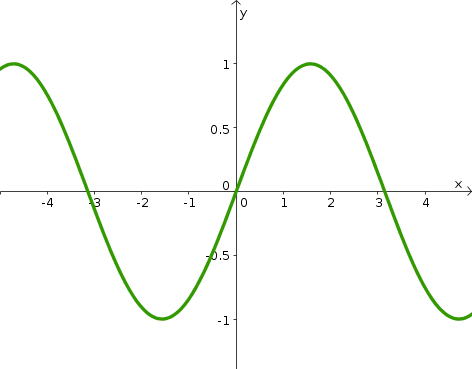
\includegraphics[width=10cm]{sinx.png}
            \caption{Gráfica de \(\sin x\).}
        \end{figure}
        \begin{figure}[H]
            \centering
            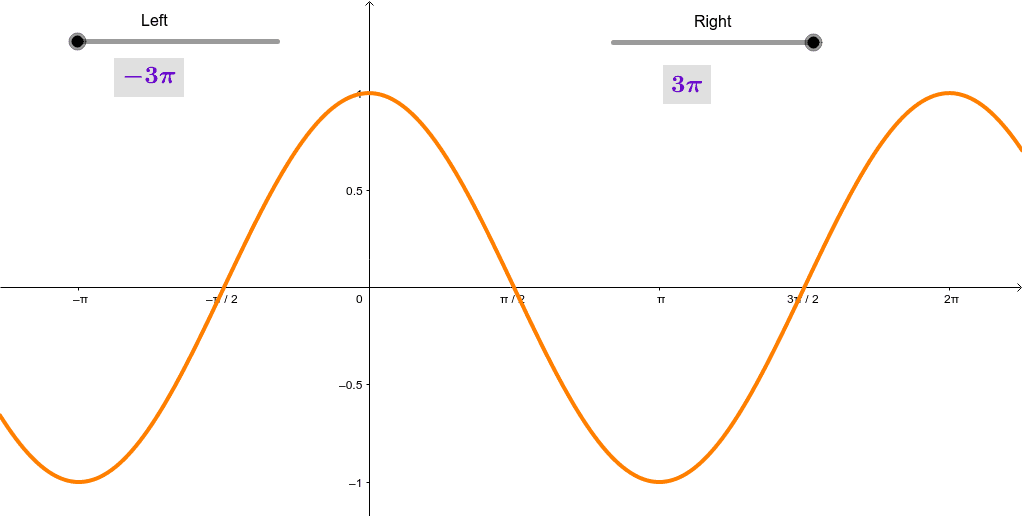
\includegraphics[width=10cm]{cosx.png}
            \caption{Gráfica de \(\cos x\).}
        \end{figure}
        \subsection{Exponenciales}
        Cuando hablamos de exponencial, nos referimos principalmente a las funciones las cuales su base es la constante \(e\) (constante de Euler), las cuales describen crecimiento exponencial (he ahí su nombre)
        \[e^x\]
        También se acostumbra a escribirla de la siguiente manera:
        \[\text{exp}\,(x)\]
        Su gráfica es la siguiente:
        \begin{figure}[H]
            \centering
            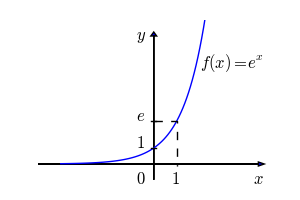
\includegraphics[width=10cm]{etothex.png}
            \caption{Gráfica de \(e^x\).}
        \end{figure}
        \subsection{Especiales}
        Unas no muy empleadas para la materia, pero igual de interesantes son las siguientes:
        \subsubsection{Gamma}
        Escrita de la manera mostrada en alusión a al letra griega mayuscula \(\Gamma\), esta función es equivalente a los factoriales de la siguiente forma:
        \[\Gamma\,(x)=(x-1)\,!\]
        Por lo tanto, si le sumamos 1, tenemos que:
        \[\Gamma\,(x+1)=(x+1-1)\,!=x\,!\]
        Esta tiene dominio en \(\mathbb{R}\) y en \(\mathbb{C}\) por lo que nos permite conocer factoriales muchos números más. Su gráfica es la siguiente:
        \begin{figure}[H]
            \centering
            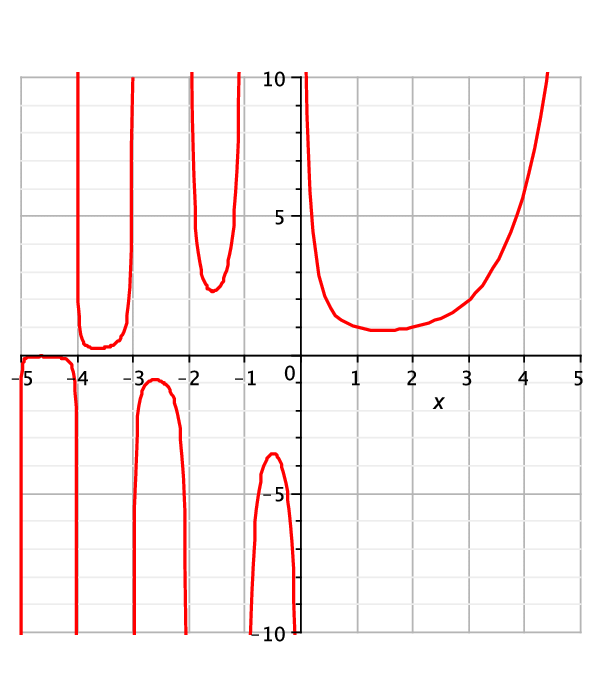
\includegraphics[width=10cm]{gammax.png}
            \caption{Gráfica de \(\Gamma\,(x)\)}
        \end{figure}
        \subsubsection{Parte fraccionaria}
        Su escritura es la siguiente:
        \[\{x\}=x-\floor*{x} , x\geq 0\]
        Y su gráfica deja picos iterados:
        \begin{figure}
            \centering
            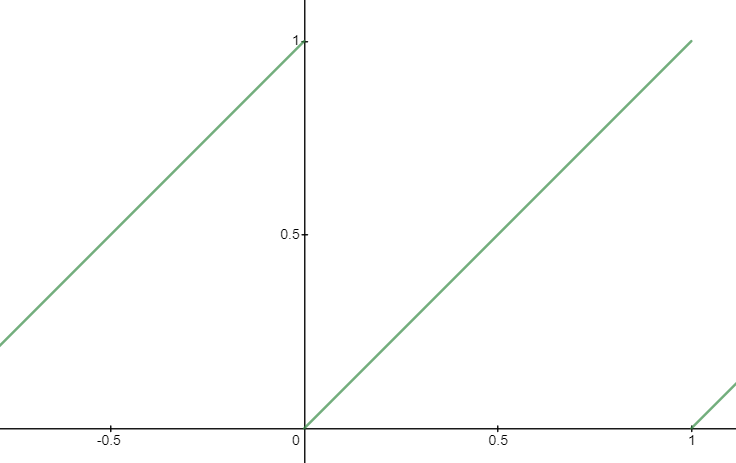
\includegraphics[width=10cm]{fracpartx.PNG}
            \caption{Gráfica de \(\{x\}\).}
        \end{figure}
        \section*{Hipervínculos de material complementario:}
        El acceso es CON CORREO INSTITUCIONAL.
        \begin{itemize}
            \item \href{https://docs.google.com/document/d/1mhFr7S5rJ7TwR297Kd6l8b6NPvYkUAlpWIxuz4VKV2w/edit?usp=sharing}{\textbf{Pizarras Online de Miro (compendio de los enlaces).}}
            \item \href{https://drive.google.com/drive/folders/1yL1gAIbVpgKB3h8498KFNE7NDZjoxIWa?usp=sharing}{\textbf{Carpeta de los Documentos PDF.}}
            \item \href{https://drive.google.com/drive/folders/1TPtNSe4ErSgaBLw2kgYDQadyXqvh6AYC?usp=sharing}{\textbf{Grabaciones de las asesorías y demás.}}
        \end{itemize}
\end{document}